\documentclass[a4paper]{article}

\usepackage{microtype}
\usepackage{url}
\usepackage[colorlinks=true]{hyperref}
\usepackage[english]{babel}
\usepackage[T1]{fontenc}
\usepackage{fancyhdr}
\usepackage{graphicx}

\title{Power Bridge Concept1}
\date{Last Updated: \today}

\begin{document}
\pagestyle{fancy} \lhead{} \rhead{}
\maketitle

\section{Power Bridge Schematic}
\begin{figure}[h!]
  \centering
  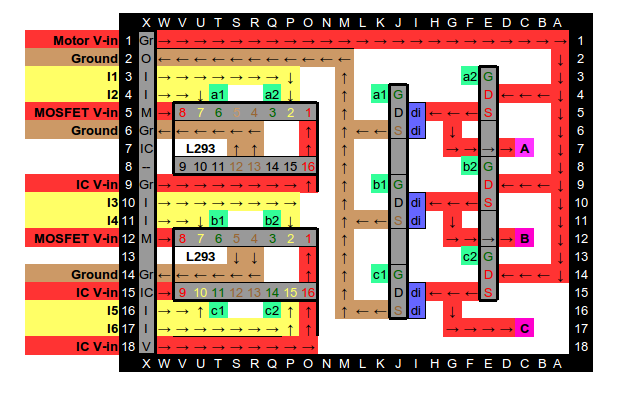
\includegraphics[width=\linewidth]{schematics/powerBridge}
\end{figure}

\section{Truth Table}
  \small
\begin{tabular}{lll|llllll|llllll} \hline
  \multicolumn{3}{c}{Output} & \multicolumn{6}{c}{MOSFET Bridge} & \multicolumn{6}{c}{Input}\\
  \hline
  A & B & C & gHA & gHB & gHC & gLA & gLB & gLC & 1 & 2 & 3 & 4 & 5 & 6 \\
  \hline
  High & Low & Null & 1 & 0 & 0 & 0 & 1 & 0 & 1 & 0 & 0 & 1 & 0 & 0\\
  High & Null & Low & 1 & 0 & 0 & 0 & 0 & 1 & 1 & 0 & 0 & 0 & 1 & 0\\
  Low & High & Null & 0 & 1 & 0 & 1 & 0 & 0 & 0 & 1 & 1 & 0 & 0 & 0\\
  Null & High & Low & 0 & 1 & 0 & 0 & 0 & 1 & 0 & 0 & 1 & 0 & 1 & 0\\
  Low & Null & High & 0 & 0 & 1 & 1 & 0 & 0 & 0 & 1 & 0 & 0 & 1 & 0\\
  Null & Low & High & 0 & 0 & 1 & 0 & 1 & 0 & 0 & 0 & 0 & 1 & 1 & 0\\
  \hline
\end{tabular}
\newpage

\section{Testing}
  \subsection{Method}
  The power bridge was connected to a \textit{Freetronics Etherten}
  microcontroller (MCU) via a \textit{breadboard}. The input signals to the power
  bridge were connected to the PWM outlets of the MCU -- pins 11, 10, 9, 6, 4
  and 3. The power bridge MOSFET and IC power buses  should be connected to a 5V
  supply, whilst the motor power bus can be connected to a larger supply (the
  test used primarily 12V, and then eventually 30V).

  The remaining digital pin outlets were connected to a 1602A LCD
  display. This was setup so that it showed the phase output readings (A, B and
  C). Note that negative values will be unsigned in the display.

  Other readings can be obtained from a multimeter.

  Uploading various programs to the MCU allows control over the power bridge
  outputs. This can also be done without the MCU, but would require manual
  reconnection of input circuitry.

  \subsection{Discussion of Results}
  \begin{enumerate}
    \item Peak phase output voltage reached approximately 12V when the motor bus
    was running at 30V (40\%)
    \item The high-side MOSFET connection for phase B was found to be weak and
    may need further soldering (done)
    \item Phases that should be \textit{null} have floating values between
    (rougly) 200 mV -- 20 mV; may need resitive loads before the MOSFETs to
    prevent floating signals.
    \item The phase output to motor bus voltage ratio is less than 1, and can be
    as low as 0.2; need to further investigate how to increase this ratio.
    \item Pushing the MOSFET deeper into the header appears to increase the
    phase output (although this is not recommended as it may lead to burns!).
    The MOSFET eventually burned out -- possibly due to a large sudden increase in
    current/voltage (12V to 30V). This may be the primary issue as to why the
    current ratio is so low -- that is, the MOSFETs are not actually entirely in
    contact with the buses. Thus a better connection method may need to be sought.
  \end{enumerate}

\section{Final Remarks}
We may need to investigate whether the low-side phase should or should not have
a negative voltage reading. A small number of tests had readings of exactly, and
steadily, 0.0 V for
their low side -- however this was difficult to duplicate in subsequent tests.

A second concept should look into fitting diodes, and snubber protection
circuits that will prevent any jump discontinuities in voltage or current.

Additionally, the second concept would be looking into designing/finding more
suitable gate drivers as the L293 are designed for H-bridges not Half H-Bridges.

\end{document}
